\chapter{CoAP resource module} \label{resourcemodule}

Nu we genoeg kennis hebben over Drupal en CoAP en een CoAP library ter beschikking hebben, kunnen we overgaan tot de uiteindelijk te ontwikkelen module. Het is deze module die een eindgebruiker zal installeren. Ze biedt dan de mogelijkheid om op een gebruiksvriendelijke en dynamische manier sensoren te bekijken en beheren van op de Drupal website, en dit zonder daarvoor technische kennis nodig te hebben van het CoAP protocol of programmatie in Drupal. We bekijken eerst globaal wat de module concreet moet aanbieden. Daarna bekijken we hoe de module in mekaar zal steken. Eens we dit weten, kunnen we overgaan tot de verschillende versies van de ontwikkelde module en de implementatie ervan.

\section{Architectuur}

\subsection{Functionaliteit}

De bedoeling van deze module is de eindgebruiker in staat te stellen om gemakkelijk sensoren toe te voegen aan zijn/haar website, ze te bekijken en te sturen. Belangrijk hierbij is dat elke Drupal gebruiker die een website maakt, deze kan gebruiken zonder extra kennis nodig te hebben over het CoAP protocol. Ook is het niet de bedoeling dat de eindgebruiker zelf nog moet programmeren in Drupal om de module te kunnen gebruiken. Kortom, de module moet out-of-the box werken en zoveel mogelijk omvatten wat mogelijk is met CoAP sensoren. Concreet houdt dit onder andere dat bij installatie van de module een content-type mee wordt ge\"{i}nstalleerd, zodat de gebruiker slechts met enkele muisklikken het content-type kan toevoegen en onmiddellijk kan beginnen met het gebruike van de sensoren. Verder worden bij installatie ook alle benodigde databanktabellen gecre\"{e}erd.\\

De configuratie die de gebruiker moet doen zoals bijvoorbeeld het toevoegen van een resource, moet gebruiksvriendelijk verlopen. Hiervoor wordt gebruik gemaakt van resource discovery, een gebruiker hoeft enkel het IPv6-adres op te geven. De sensoren die aangesloten zijn op dat embedded device worden dan opgesomd voor de gebruiker, die dan de mogelijk krijgt de sensoren aan te vinken om ze toe te voegen aan de website.\\
Dit principe wordt zelfs verder doorgetrokken. Een gebruiker zal tevens de mogelijkheid krijgen om alle embedded devices in een subnetwerk op te vragen. Dit gebeurt aan de hand van een resource directory waarin alle well-known/core's van de embedded devices in het subnetwerk zich bevinden. De gebruiker krijgt dan de kans een embedded device te kiezen om dan resources te selecteren.\\

Eens de gebruiker de gewenste resources heeft toegevoegd aan zijn/haar website, is het de bedoeling dat de 4 REST-methodes GET, PUT, POST, DELETE kunnen uitgevoerd worden, op voorwaarde dat de desbetreffende sensor de methode ondersteunt (dit wordt weergegeven bij het toevoegen van sensoren). Naast deze methodes kan een sensor ook nog observable zijn (zie hoofdstuk \ref{CoAP}), de gebruiker moet dus ook in staat gesteld worden om sensoren te observen.









%---------------------------------------- ALLES HIERNA IS NOG NIET VERWERKT ------------------------------------------------------------

Er moet een module ontwikkeld worden voor Drupal die de gebruiker in staat moet stellen sensoren te kunnen beheren, waarbij als onderliggend protocol CoAP wordt gebruikt. De module moet zo veel mogelijk out-of-the-box te gebruiken zijn, wat inhoudt dat zoveel mogelijk benodigdheden mee ge\"{i}nstalleerd worden zonder extra tussenkomst van de gebruiker. Concreet betekent dit dat de benodigde content-types, zowel voor de gebruiker als de tabellen voor de databank, automatisch mee ge\"{i}nstalleerd worden bij installatie van de module.\\

Het content-type aan gebruikerskant moet de mogelijkheid bieden om dynamisch aan te geven welke sensoren hij/zij wil beheren en in welk vorm de data moet aangeboden worden. De gebruiker kan zelf een URI opgeven, maar nieuwe sensoren moeten automatisch gedetecteerd worden en beschikbaar gesteld worden aan de gebruiker aan de hand van een resource directory.\\

Een gebruiker moet een waarde kunnen ophalen met een GET-request maar, indien de sensor dit ondersteunt, moet het ook mogelijk zijn zich in te schrijven bij de sensor om hem te observeren. Hierbij pusht de sensor op eigen initiatief de data naar de ge\"{i}nteresseerden.\\

Wanneer een sensor de PUT-methode ondersteunt moet de gebruiker deze ook kunnen uitvoeren.


De gebruiker moet in staat zijn om:

\begin{itemize}
\item cores op te vragen;
\item de vier REST-methodes op een resource aan te roepen;
\end{itemize}

\section{Evolutie}

We kunnen de evolutie van deze module opsplisten in volgende stappen (niet klaar):

\begin{enumerate}
\item temperatuurmodule met HTTP/CoAP-proxy, GET en observe worden meteen ondersteund;
\item temperatuurmodule met native CoAP;
\item module maakt gebruik van externe CoAP library en ondersteunt verschillende content-types;
\item module ondersteunt resource discovery van ��n device en cre\"{e}ert een custom content-type bij installatie
\item module ondersteunt de drie andere REST methodes (PUT, POST en DELETE)
\item module ondersteunt resource discovery van meerdere devices en laat toe custom lijsten samen te stellen van resources verspreid over verschillende devices;
\item module ondersteunt het gebruik van een resource directory;
\item ...
\item finale module.
\end{enumerate}

\section{Temperatuurmodule met HTTP/CoAP-proxy}

In deze paragraaf wordt besproken hoe de temperatuurmodule wordt gemaakt die gebruik maakt van een HTTP/CoAP-proxy. Bovendien wordt ook aangetoond hoe waarden opgeslagen worden in de databank om de geschiedenis van opvragingen bij te houden.\\

De gebruiker klikt op een knop die het automatisch periodiek bevragen van een embedded device initialiseert. Periodiek wordt een HTTP GET-request naar een HTML-pagina uitgevoerd. Wanneer de response ontvangen wordt, wordt de HTML-pagina geparsed, waarna de nuttige informatie in de databank wordt geplaatst. Met jQuery worden dan nieuwe waarden opgehaald en getoond aan de gebruiker.

\begin{figure}[h]
\vspace{10pt}
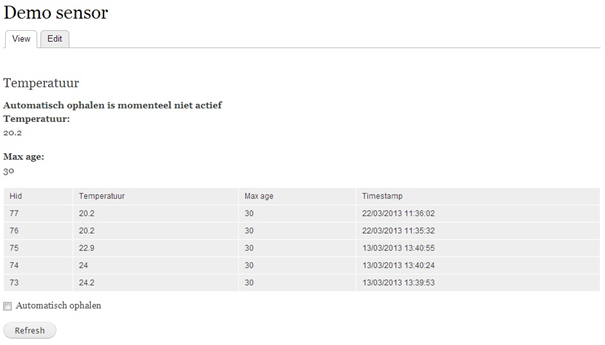
\includegraphics[width=1\textwidth]{fig/TemperatuurModuleHTTPCOAPProxy}
\vspace{-30pt}
\caption{Temperatuurmodule met HTTP/COAP-proxy}
\vspace{-10pt}
\end{figure}

\subsection{Proxy}

Als proxy werd de coap.me website gebruikt van iMinds. Deze biedt de mogelijkheid om de notificaties van een embedded device te bekijken in een browser. De website biedt ook de mogelijkheid om door te klikken naar de notificatie om die volledig te bekijken op een pagina.\\

Het is deze laatste pagina die periodiek wordt opgehaald en geparsed. De communicatie vanwege de Drupal-module bestaat dus enkel uit HTTP-communicatie, de proxy verzorgt de nodige CoAP-berichten tussen zichzelf en het embedded device.

\subsection{Achtergrondprocessen}

In een eerste fase van deze module werd er gebruik gemaakt van een formulier en werd bij het indienen van dit formulier, eerst de request uitgevoerd en dan gewacht op de response om de nieuwe pagina op te bouwen. Het spreekt voor zich dat dit geen goed oplossing is, daar de gebruiker zal moeten wachten op de pagina wanneer de communicatie traag is of misloopt, de gebruiker kan snel het idee krijgen dat er geen verbinding meer is met de website.\\

In het vorige hoofdstuk zagen we dat een mogelijke oplossing het gebruik van jQuery is. In deze situatie is jQuery echter geen goede optie, daar jQuery de databank van Drupal niet zomaar kan manipuleren. Hiervoor zouden een connectiestring, wachtwoord en dergelijke gegevens nodig zijn, en jQuery van die informatie voorzien is een grote bedreiging voor de veiligheid, bovendien zou dit een oplossing zijn met een zeer sterke koppeling, wat nooit een goed idee is.\\

De gebruikte oplossing illustreert alweer de voordelen van een open source platform met een uitgebreide community. Er is namelijk al een Background Process module gemaakt in het verleden, het zou dus zonde zijn om hier niet dankbaar gebruik van te maken. Zoals de naam suggereert, biedt de Background Process module de mogelijkheid om achtergrondprocessen op te starten. Deze draaien op de achtergrond op de server en storen dus geen andere processen zoals het opbouwen van een pagina voor de gebruiker, waardoor de gebruiker dus niet geconfronteerd wordt met lange wachttijden.\\

Sterker nog, er is ook een functie voorzien om een HTTP GET-request uit te voeren, waarbij je een callback-functie opgeeft. Wanneer er een response is, zal dus automatisch de opgegeven functie opgeroepen worden met de response als argument.

\subsection{Geschiedenis van opvragingen}

Alles is nu voorhanden om een geschiedenis bij te houden van opgevragen waarden. Het achtergrondproces kan ongestoord op de server periodiek een GET-request uitvoeren en omdat dit op de server gebeurt kunnen de waarden gemakkelijk en dynamisch toegevoegd worden aan de databank.\\

Er rest ons nu enkel nog een manier te vinden om de client op de hoogte te brengen van nieuwe waarden en hem van die waarden te voorzien.\\

Op deze manier staat het ophalen van waarden en die in de databank stoppen los van het tonen van diezelfde waarden aan de client. Dit zorgt ervoor dat een andere gebruiker evengoed ook de waarden kan bekijken, er is dus een ��n-naar-veel relatie.

\subsection{Push-strategie: node.js}

De mooiste oplossing en tevens ��n met het minste aandeel aan overhead, is een oplossing waarbij de server zelf op eigen initiatief data kan sturen naar de client. Hierbij is dan geen polling-mechanisme nodig door de client, wat de netwerkbelasting drastisch verlaagt en de verantwoordelijkheid verschuift naar de server.\\

Om een push-strategie te verwezenlijken werd een uitgebreide literatuurstudie van node.js uitgevoerd. Node.js is een javascript-library die je in staat stelt bi-directioneel verkeer te verwezenlijken. Hierbij wordt gebruik gemaakt van kanalen die worden opgezet, zo?n kanaal kan dan door beide partijen gebruikt worden.\\

Concreet zou het in de context van deze masterproef mogelijk zijn om met node.js een JavaScript-functie op te roepen bij de client op initiatief van de server.\\

Er is meermaals gepoogd dit te realiseren, maar de summiere documentatie van node.js laat op sommige vlakken te wensen over. Zo zijn we er niet in geslaagd documentatie te vinden over het opzetten van een eigen kanaal of een bestaand kanaal te gebruiken.\\

Bovendien is het nodig voor node.js om een extra server te draaien waarlangs het verkeer moet passeren. Aangezien het vaak niet mogelijk is om de shell van de webserver te gebruiken in een free-hosting omgeving, is dit een erg groot nadeel.
Er bestaan wel servers die je kan gebruiken, maar dit tegen betaling.\\

Wij, als ontwikkelaar van de module, kunnen niet verwachten dat een eindgebruiker een extra server ter beschikking heeft of dat zelfs wilt. Het is de bedoeling dat onze module zo veel mogelijk out-of-the-box bruikbaar is.\\

Vandaar dat wij geopteerd hebben geen gebruik te maken van node.js en dus ook niet van een push-strategie.

\subsection{Pull-strategie}

Aangezien een push-strategie niet of moeilijk kan gebruikt worden, hebben wij gekozen voor een pull-oplossing.\\

Uiteraard was de eerste reactie gebruik te maken van de Drupal-community en dus te zoeken in de vele modules die beschikbaar zijn. Er is tot op heden geen module geschreven door iemand anders in de Drupal-community dat ons probleem behandelt. De inspiratie voor de uiteindelijke oplossing werd wel gehaald uit een bestaande module, namelijk de Block Refresh-module.\\

Deze laatste maakt gebruik van jQuery en AJAX calls om periodiek de inhoud van een block te refreshen, waarbij je zelf de lengte van de periode kan bepalen. In jQuery loopt een timer die periodiek een JavaScript-functie oproept. In deze functie wordt dan een AJAX call uitgevoerd naar de Drupal server, die op zijn beurt een antwoord terug stuurt.\\

Hetzelfde mechanisme wordt gebruikt in onze module.
Wanneer de pagina geladen wordt bij de client, start een timer die periodiek een AJAX call uitvoert naar de Drupal server. Op de Drupal server is een AJAX callback functie gedefinieerd aan de hand van de hook hook\_menu(). Deze hook wordt gebruikt om menu items toe te voegen aan de site en om AJAX callbacks te definieren.\\

De callback-functie haalt dan de laatst toegevoegde rij op en stuurt volgende kolommen naar de client:

\begin{itemize}
\item Hid: een History-id die de opvragingen onderscheidt
\item Temperatuur: de effectieve waarde in graden Celsius.
\item Max age: De geldigheidsperiode van de waarde in seconden.
\item Timestamp: Het tijdstip van opvragen.
\end{itemize}
	
In de jQuery-functie bij de client wordt dan het opgehaalde history-id vergeleken met de hoogste history-id in de tabel op de pagina.
Als de opgehaalde waarde nieuwer is dan die op de pagina, wordt de nieuwe rij ingevoegd bovenaan de tabel op de pagina.

\section{Temperatuurmodule met native CoAP}

